\section{Results}
\label{sec:results}

Table~\ref{tab:main} and Figure~\ref{fig:leaderboard} report the score of every system on the 500 instances of VBVR-Pro-Bench (video setting): the three closed-model coding agents, the 23 open-weight models run through OpenCode, and the eleven video models of the published leaderboard~\citep{vbvrpro2026}. All 37 systems are scored by the same unmodified official evaluator, and an instance with no video counts 0. Every number in this section is produced by \texttt{paper/figures/make\_figures.py} from the released result files.

% Generated by paper/figures/make_figures.py from bench/paper/table1_leaderboard.csv and bench/results/ -- do not edit by hand.
\begin{table*}[t]
\centering
\caption{VBVR-Pro-Bench (video setting, 100 tasks $\times$ 5 instances) leaderboard. Every system is scored by the unmodified official rule-based evaluator of the benchmark kit; the score is the mean over all 500 instances, and an instance for which the system produced no video counts 0. Coding-agent rows are our runs (one attempt per instance, sandboxed, no image or video model available); video-model rows are the published VBVR-Pro leaderboard numbers~\citep{vbvrpro2026}, not rerun by us. \emph{Rank} is the position among all 37 systems. \emph{Videos} is the number of instances for which the agent wrote a video file (--- for video models, which we did not run). In-domain (ID) tasks are the 50 families with training data in VBVR-Pro, out-of-domain (OOD) the 50 families held out from all training. Best per column in bold, second underlined; the best coding agent and the best video model are shaded. $^\dagger$No video in any of the 500 attempts (the model answers in prose and never calls a tool).}
\label{tab:main}
\small
\setlength{\tabcolsep}{5pt}
\begin{tabular}{rlcccc}
\toprule
Rank & System & Overall & ID & OOD & Videos / 500 \\
\midrule
\multicolumn{6}{l}{\emph{Coding agents, closed models}} \\[1pt]
\rowcolor{bestcolor} 1 & Codex (gpt-6-astra) & \textbf{0.923} & \textbf{0.879} & \textbf{0.967} & 500 \\
2 & Claude Code (Fable 5.1) & \underline{0.894} & \underline{0.830} & 0.958 & 500 \\
3 & Gemini CLI (Gemini 3.1 Pro) & 0.893 & 0.826 & \underline{0.960} & 500 \\
\midrule
\multicolumn{6}{l}{\emph{Coding agents, open-weight models (OpenCode)}} \\[1pt]
5 & GLM-5 & 0.572 & 0.479 & 0.664 & 495 \\
7 & Kimi K2.5 & 0.557 & 0.454 & 0.660 & 498 \\
11 & MiniMax M2.5 & 0.451 & 0.386 & 0.515 & 488 \\
14 & DeepSeek V3.2 & 0.378 & 0.303 & 0.452 & 475 \\
15 & Devstral 2 123B & 0.350 & 0.275 & 0.426 & 494 \\
16 & Kimi K2 Thinking & 0.313 & 0.218 & 0.407 & 406 \\
18 & gpt-oss-120b & 0.270 & 0.196 & 0.344 & 380 \\
19 & Qwen3-Coder-Next & 0.264 & 0.218 & 0.310 & 498 \\
20 & Nemotron Super 3 120B & 0.200 & 0.139 & 0.261 & 436 \\
22 & Qwen3-Coder-30B-A3B & 0.143 & 0.099 & 0.186 & 480 \\
23 & Mistral Large 3 675B & 0.127 & 0.079 & 0.176 & 254 \\
25 & GLM-4.7-Flash & 0.104 & 0.081 & 0.127 & 470 \\
27 & gpt-oss-20b & 0.079 & 0.075 & 0.083 & 148 \\
28 & Qwen3-Next-80B-A3B & 0.070 & 0.034 & 0.105 & 167 \\
29 & Llama 4 Scout & 0.049 & 0.040 & 0.058 & 269 \\
30 & Nemotron Nano 3 30B & 0.028 & 0.026 & 0.029 & 91 \\
31 & Qwen3-VL-235B-A22B & 0.025 & 0.022 & 0.028 & 70 \\
32 & Qwen3-32B & 0.004 & 0.006 & 0.003 & 25 \\
33 & Llama 4 Maverick & 0.001 & 0.001 & 0.002 & 7 \\
34 & Gemma 3 27B & 0.000 & 0.000 & 0.000 & 0$^\dagger$ \\
35 & Gemma 3 12B & 0.000 & 0.000 & 0.000 & 0$^\dagger$ \\
36 & Magistral Small & 0.000 & 0.000 & 0.000 & 0$^\dagger$ \\
37 & Llama 3.3 70B & 0.000 & 0.000 & 0.000 & 0$^\dagger$ \\
\midrule
\multicolumn{6}{l}{\emph{Video models (VBVR-Pro leaderboard)}} \\[1pt]
\rowcolor{secondcolor} 4 & VBVR-Pro-Wan2.2-I2V-A14B (RL) & 0.670 & 0.808 & 0.532 & --- \\
6 & VBVR-Pro-Wan2.1-I2V-14B & 0.562 & 0.730 & 0.395 & --- \\
8 & VBVR-Wan2.2 & 0.517 & 0.548 & 0.486 & --- \\
9 & Seedance 2.0 & 0.499 & 0.451 & 0.547 & --- \\
10 & VBVR-Pro-Wan2.2-TI2V-5B & 0.470 & 0.641 & 0.300 & --- \\
12 & VBVR-Pro-LTX2.3 & 0.425 & 0.527 & 0.324 & --- \\
13 & Kling VIDEO 3.0 & 0.392 & 0.356 & 0.427 & --- \\
17 & Veo 3.1 & 0.309 & 0.312 & 0.305 & --- \\
21 & Wan2.2-I2V-A14B & 0.182 & 0.157 & 0.207 & --- \\
24 & LTX-2.3-I2AV & 0.112 & 0.106 & 0.119 & --- \\
26 & Wan2.1-I2V-14B-720P & 0.100 & 0.105 & 0.095 & --- \\
\bottomrule
\end{tabular}
\end{table*}


\begin{figure}[!t]
\centering
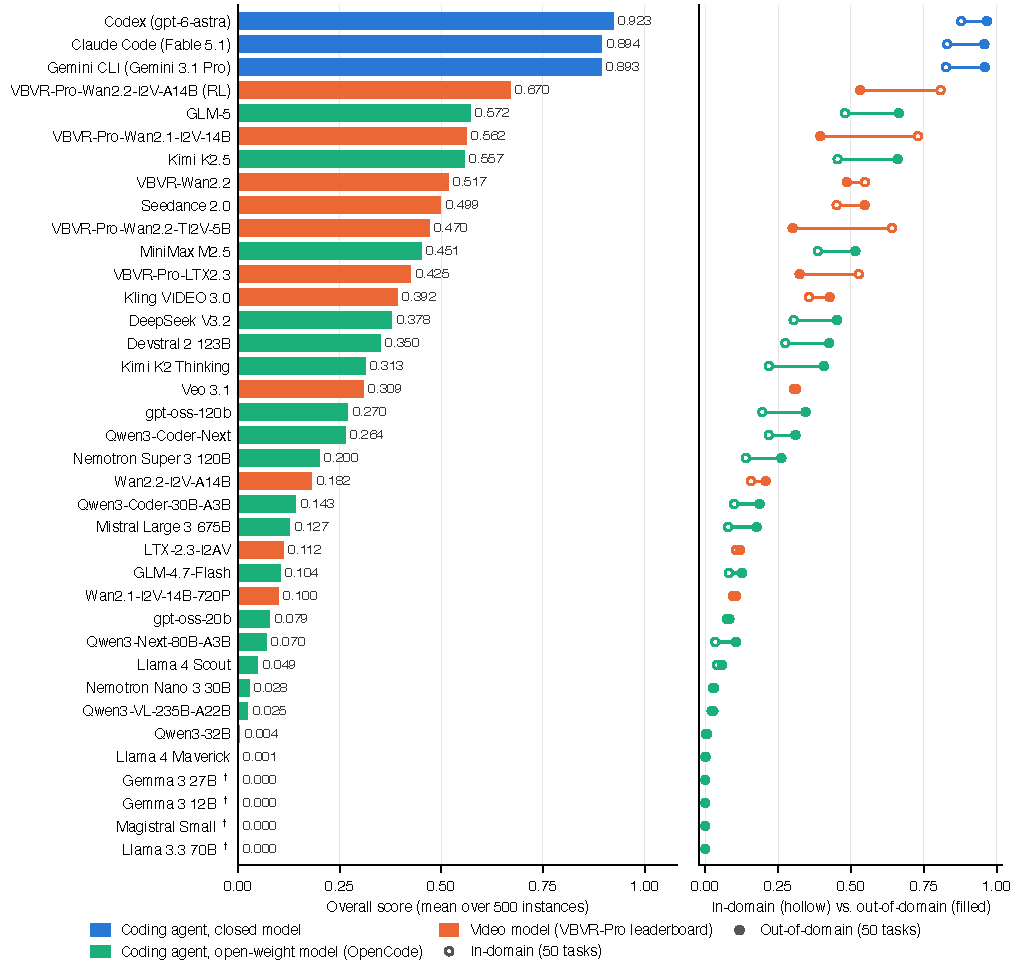
\includegraphics[width=\textwidth]{figures/fig_leaderboard.pdf}
\caption{The 33 systems that produced at least one video, sorted by overall score (bar: mean over the 500 instances, coloured by system class), with the in-domain score as a hollow circle and the out-of-domain score as a solid diamond on each bar and a dashed line at the best video model (0.670). For every coding agent above the noise floor the diamond lies to the right of the circle, and for every video model trained on the benchmark's task families it lies to the left. The four systems with no video in 500 attempts are named below the axis.}
\label{fig:leaderboard}
\end{figure}

\subsection{Main Comparison}
\label{sec:res-main}

The three closed-model coding agents occupy the top three positions. Codex with gpt-6-astra scores 0.923, Claude Code with Fable~5.1 scores 0.894, and Gemini CLI with Gemini~3.1~Pro scores 0.893, all with a video on 500 of 500 instances. The best video model, VBVR-Pro-Wan2.2-I2V-A14B, which was RL-trained on the in-domain task families with the same evaluator as reward, scores 0.670. The gap between the best agent and the best video model is 0.253; the second-best video model, VBVR-Pro-Wan2.1-I2V-14B, is a further 0.108 behind at 0.562. The three agents are within 0.030 of each other, so the result does not hinge on one model.

The gap is not an evaluator artefact. The checker is the benchmark's own, run unchanged, and the video-model rows are the authors' numbers with the same checker. The agents never see the ground truth, the generator or the task metadata, and have no image or video model. Each writes a program that reads the first frame, computes the answer and renders it.

\subsection{In-Domain versus Out-of-Domain}
\label{sec:res-ood}

The benchmark splits its 100 tasks into 50 in-domain families, for which VBVR-Pro provides training data, and 50 out-of-domain families held out from all training. Figure~\ref{fig:ood} plots OOD minus ID for every system that produced at least one video. The two classes move in opposite directions.

\begin{wrapfigure}{r}{0.48\textwidth}\vspace{-8pt}
\centering
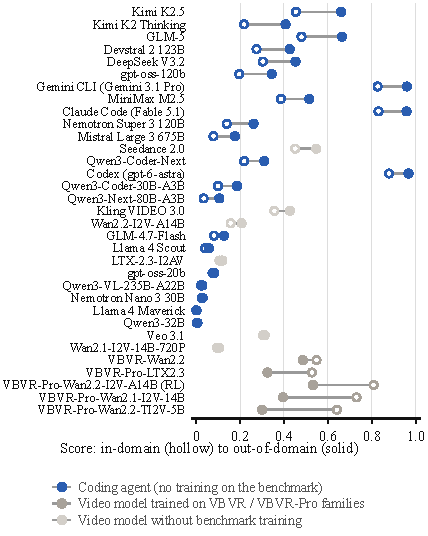
\includegraphics[width=\linewidth]{figures/fig_ood.pdf}
\caption{In-domain score (hollow) and out-of-domain score (solid) of every system with at least one video, sorted by the difference between the two. Coding agents (blue), none trained on the benchmark, gain on the held-out families; the five video models trained on VBVR or VBVR-Pro task families (grey) lose between 0.062 and 0.341, and video models without benchmark training (light grey) sit near zero. Values are the ID and OOD columns of Table~\ref{tab:main}.}
\label{fig:ood}\vspace{-8pt}
\end{wrapfigure}
Coding agents score higher out of domain. Codex goes from 0.879 in domain to 0.967 out of domain ($+0.089$), Claude Code from 0.830 to 0.958 ($+0.128$), Gemini CLI from 0.826 to 0.960 ($+0.133$). The open-weight models gain more: GLM-5 $+0.185$, Kimi~K2.5 $+0.206$. Of the 22 coding agents with a video, 21 have a positive difference; the exception, Qwen3-32B, produced 25 videos and scores 0.006 versus 0.003 ($-0.003$, noise). No agent was trained on any family, so the split has no meaning for them. The held-out families are simply easier for a program; 11 of the 12 hardest tasks for the closed agents are in-domain (Table~\ref{tab:hardest}).

Video models trained on the benchmark score lower out of domain. All five VBVR- and VBVR-Pro-trained models drop: VBVR-Pro-Wan2.2-I2V-A14B from 0.808 to 0.532 ($-0.276$), VBVR-Pro-Wan2.1-I2V-14B from 0.730 to 0.395 ($-0.335$), VBVR-Pro-Wan2.2-TI2V-5B from 0.641 to 0.300 ($-0.341$), VBVR-Pro-LTX2.3 from 0.527 to 0.324 ($-0.203$), VBVR-Wan2.2 from 0.548 to 0.486 ($-0.062$). The video models without benchmark training are flat or slightly up: Seedance~2.0 $+0.096$, Kling~3.0 $+0.071$, Wan2.2-I2V-A14B $+0.050$, LTX-2.3-I2AV $+0.013$, Veo~3.1 $-0.007$, Wan2.1-I2V-14B-720P $-0.010$. Training a video model on the task families buys in-domain score at the cost of out-of-domain score. The RL-trained A14B is the only video model above 0.8 in domain, and out of domain it falls to 0.532, below Seedance~2.0 (0.547), which never saw the benchmark. Out of domain every closed agent is above 0.95 and the best video model is at 0.547. In domain the agents still lead, with Codex at 0.879, Claude Code at 0.830 and Gemini CLI at 0.826 against 0.808 for the A14B, on the split it was trained on with the evaluator as its reward.

\subsection{Results by Category}
\label{sec:res-category}

Table~\ref{tab:categories} breaks the score down by the benchmark's five task categories: Abstraction (25 tasks), Perception (28), Spatiality (16), Transformation (12) and Knowledge (19). The closed agents are above 0.8 in every category. Codex is best on Abstraction (0.957) and Knowledge (0.863), Gemini CLI on Perception (0.972), and Claude Code on Spatiality (0.908) and Transformation (0.943). The lowest closed-agent cell is Gemini CLI on Spatiality (0.816), the highest Gemini CLI on Perception (0.972).

% Generated by paper/figures/make_figures.py from bench/paper/table2_categories.csv -- do not edit by hand.
\begin{table*}[t]
\centering
\caption{Coding-agent score by task category (mean over the 5 instances of every task in the category, both splits; the number of tasks per category is in the second header row). The three closed-model agents and the eight best open-weight models are shown; best per column in bold, second underlined. The last row is the in-domain category profile of the released VBVR-Pro baseline video model as reported in the VBVR-Pro paper~\citep[Table~8]{vbvrpro2026}; because it covers the 50 in-domain tasks only, the block above it restricts the three closed-model agents to the same 50 tasks (task counts per category in that block's header row; computed from the per-instance results). Rows in the in-domain block are not ranked.}
\label{tab:categories}
\small
\setlength{\tabcolsep}{4pt}
\begin{tabular}{lcccccc}
\toprule
System & Abstraction & Perception & Spatiality & Transformation & Knowledge & Overall \\
\emph{Tasks per category} & (25) & (28) & (16) & (12) & (19) & (100) \\
\midrule
\multicolumn{7}{l}{\emph{Coding agents, closed models}} \\[1pt]
Codex (gpt-6-astra) & \textbf{0.957} & 0.953 & \underline{0.903} & \underline{0.902} & \textbf{0.863} & \textbf{0.923} \\
Claude Code (Fable 5.1) & 0.838 & \underline{0.957} & \textbf{0.908} & \textbf{0.943} & 0.834 & \underline{0.894} \\
Gemini CLI (Gemini 3.1 Pro) & \underline{0.878} & \textbf{0.972} & 0.816 & 0.894 & \underline{0.861} & 0.893 \\
\midrule
\multicolumn{7}{l}{\emph{Coding agents, open-weight models (OpenCode)}} \\[1pt]
GLM-5 & 0.478 & 0.748 & 0.491 & 0.569 & 0.506 & 0.572 \\
Kimi K2.5 & 0.427 & 0.727 & 0.527 & 0.582 & 0.490 & 0.557 \\
MiniMax M2.5 & 0.347 & 0.633 & 0.412 & 0.439 & 0.358 & 0.451 \\
DeepSeek V3.2 & 0.308 & 0.538 & 0.358 & 0.288 & 0.307 & 0.378 \\
Devstral 2 123B & 0.290 & 0.478 & 0.382 & 0.296 & 0.248 & 0.350 \\
Kimi K2 Thinking & 0.231 & 0.476 & 0.359 & 0.195 & 0.216 & 0.313 \\
gpt-oss-120b & 0.224 & 0.348 & 0.300 & 0.167 & 0.255 & 0.270 \\
Qwen3-Coder-Next & 0.260 & 0.364 & 0.195 & 0.180 & 0.232 & 0.264 \\
\midrule
\multicolumn{7}{l}{\emph{In-domain tasks only}} \\[1pt]
\emph{Tasks per category} & (13) & (7) & (10) & (6) & (14) & (50) \\
Codex (gpt-6-astra) & 0.928 & 0.948 & 0.872 & 0.823 & 0.826 & 0.879 \\
Claude Code (Fable 5.1) & 0.763 & 0.931 & 0.874 & 0.905 & 0.780 & 0.830 \\
Gemini CLI (Gemini 3.1 Pro) & 0.817 & 0.910 & 0.767 & 0.848 & 0.826 & 0.826 \\
VBVR-Pro-Wan2.2-TI2V-5B (video model) & 0.578 & 0.476 & 0.480 & 0.724 & 0.511 & 0.641 \\
\bottomrule
\end{tabular}
\end{table*}


The open-weight models have a different profile. Perception is their strongest category by a wide margin (GLM-5 0.748, Kimi~K2.5 0.727, MiniMax~M2.5 0.633), Abstraction and Knowledge the weakest (GLM-5 0.478 and 0.506). Reading the first frame correctly is within reach of the mid-tier models; the categories that need a multi-step plan separate them from the closed models.

The only published per-category numbers for a video model are those of the VBVR-Pro-Wan2.2-TI2V-5B baseline~\citep[Table~8]{vbvrpro2026}. We compare against its in-domain profile, and the last block of Table~\ref{tab:categories} restricts the closed agents to the same 50 tasks. All three agents lead the baseline in every category. Codex leads it by 0.099 on Transformation (0.823 versus 0.724), the video model's best category, and by 0.472 on Perception (0.948 versus 0.476), its worst, which is the strongest category of all three agents (0.910 to 0.948).

\subsection{Open-Weight Models}
\label{sec:res-open}

The best open-weight coding agent beats every video model except the RL-trained one. GLM-5 through OpenCode scores 0.572, fifth among all 37 systems, above VBVR-Pro-Wan2.1-I2V-14B (0.562), VBVR-Wan2.2 (0.517), Seedance~2.0 (0.499) and the seven video models below them; only the RL-trained A14B (0.670) is ahead. Kimi~K2.5 (0.557) is seventh. Out of domain, GLM-5 (0.664) and Kimi~K2.5 (0.660) are above every video model, whose best OOD score is 0.547.

The open-weight ranking is a ranking of agentic coding ability. Scores fall from GLM-5 (0.572) through MiniMax~M2.5 (0.451) and DeepSeek~V3.2 (0.378) to a long tail below 0.3, and the \emph{Videos} column of Table~\ref{tab:main} tracks the drop. The top six wrote a video on 406 to 498 of 500 instances, Mistral~Large~3 on 254, gpt-oss-20b on 148, Qwen3-32B on 25, Llama~4~Maverick on 7. Gemma~3~27B, Gemma~3~12B, Magistral~Small and Llama~3.3~70B produced no video in 500 attempts and score 0, by the same rule that scores a video model that fails to generate. Table~\ref{tab:efficiency} traces these failures to tool use; the four zero lanes never call a tool and answer in prose. Whether a lane beats the trained video models or scores 0 turns first on whether the model runs a program at all.
